\section{Verificación de la suite de simulación}

En este capítulo se verán resultados en base a la elección de parámetros y datos de un CubeSat operativo, para obtener los MoP de apuntamiento con sus respectivos costos según los niveles de componentes físicos impuestos dentro de la simulación. Para ello, se define la cuantificación de los MoP de apuntamiento, se entregan los parámetros orbitales y se observan los valores obtenidos.

\subsection{Cuantificación de los MoP de apuntamiento}

Para lograr una capacidad de apuntamiento óptima, se debe considerar los MoP de apuntamiento. El apuntamiento se define como la capacidad que tiene el CubeSat para orientar la carga útil hacia un objetivo en específico, el cual, para este proyecto, será la tierra al imponer misiones del tipo observación terrestre. Teniendo esto en cuenta, existen índices de rendimiento con los cuales se verifica si este apuntamiento del satélite fue un éxito o un fracaso. Estos fueron revisados y descritos cualitativamente en \cite{ref6}, y debido a una revisión bibliográfica más extensa en libros sobre diseño de ADCS, se corrigieron y se cuantificaron, quedando como se muestra a continuación:

\underline{Exactitud de apuntamiento \cite{ref5,ref7}}

Es el índice con mayor relevancia dentro de las misiones de observación terrestre y de apuntamiento en general. Se refiere al error absoluto de apuntamiento del satélite, por lo que es la capacidad del CubeSat de mantener y controlar su orientación hacia una sección especifica de la Tierra. Esta se mide en termino de grados sexagesimales [°] o radianes [rad] y se notará dicho valor como la resta entre la orientación deseada del CubeSat y la posición obtenida mediante el ADCS, sabiendo que existen posibles errores de determinación de actitud o de actuadores que no puedan ejercer el torque requerido.

\underline{Jitter \cite{ref5,ref9,ref10}}

El Jitter en la línea de visión (LoS, por sus siglas en inglés) de la nave espacial se define como las vibraciones mecánicas sinusoidales de pequeña amplitud que ocurren debido a las interacciones dinámicas causadas por dispositivos mecánicos vibratorios montados en la nave espacial o dentro del instrumento (s) de carga útil y que aparecen a frecuencias en o por encima del ancho de banda del Attitude Control System (ACS) del satélite, desde unos pocos Hz hasta cientos de Hz, y que perturban indeseablemente el apuntamiento de la línea de visión de la carga útil. 

Para visualizar este problema, se debe revisar si existen en las sinusoidales alrededor del eje de equilibrio a controlar en los ángulos de Euler, leves perturbaciones asemejadas al ruido, que representan la inestabilidad del satélite al tomar diferentes orientaciones pequeñas en bajos periodos de tiempo, que hacen que la cámara sea vea “empañada”. Para representar dicho problema, se considera la densidad espectral de potencia como una medida de cuantificación del jitter, el cual se obtendrá una vez fijado un filtro pasa alto de hasta una frecuencia adecuada (generalmente 10 [Hz]) aplicada a la respuesta obtenida. Se observará un alto nivel de jitter si existe un valor de la densidad espectral de potencia mayor, al consumir más energía en dicho rango de frecuencias.


\underline{Agilidad \cite{ref5, ref11}}

Se refiere a lograr una maniobra de actitud mínima, el cual es una combinación de apuntar al objetivo (sección de la Tierra) en el menor tiempo posible a través de una maniobra de giro. En otras palabras, se busca que el CubeSat intercepte al objetivo lo más rápido posible y mantenga la orientación en una exactitud de apuntamiento aceptable dentro de los requerimientos.

Para cuantificar este índice, se hará uso del parámetro del tiempo de asentamiento (Settling Time), el cual especifica el tiempo permitido para recuperarse de maniobras o perturbaciones. Si existe un tiempo de asentamiento menor en alguna comparación de dos ADCS, sería más ágil aquel que presente un menor tiempo de asentamiento, comparándolo a través de una gráfica de velocidad angular respecto al tiempo, asumiendo una banda de asentamiento adecuada.

\underline{Drift \cite{ref5}}

Se refiere a cuánto puede desviarse un vehículo con el tiempo. Este parámetro es crucial cuando se necesita mantener una dirección específica y se deben hacer correcciones solo ocasionalmente para evitar que el vehículo se desvíe significativamente de su curso deseado. Representado mediante ángulos por hora [°/hr].

Para el caso de este análisis de la suite de simulación, se consideraron solo las tres primeras. El Drift solo se menciona, pero no se cuantifica en este trabajo.

\subsection{Condiciones y parámetros de simulación}

Para obtener resultados de rendimiento, se utilizaron los datos de TLE del SUCHAI-3 con fecha de inicio del 01 de noviembre del 2023, que son las mismas condiciones iniciales utilizadas en el Capítulo 4 para visualizar el SGP4 y los modelos orbitales en ECI (IGRF y vector sol). Se debe tener en cuenta que estas condiciones, en conjunto con otros parámetros son dados para todos los niveles de sensores y actuadores impuestos dentro de la suite de simulación, y sirven para tener un parámetro comparativo entre los componentes físicos del ADCS.

En la Tabla~\ref{tab:parametros} se muestran los valores de los parámetros recién mencionados utilizados en la simulación, que son basados en literatura \cite{ref14,ref41,ref44} o por elaboración propia. Cabe mencionar que $q_i$ y $\omega_i$ representan la orientación y velocidad angular inicial real.

\begin{table}[h!]
	\centering
	\caption{Parámetros del sistema}
	\begin{tabular}{|c|c|}
		\hline
		\textbf{Parámetro} & \textbf{Valor} \\
		\hline
		$[I_x, I_y, I_z] \ [kg \cdot m^2]$ & $[0.037, 0.036, 0.036]$ \\
		\hline		
		$[I_{s0}, I_{s1}, I_{s2}] \ [kg \cdot m^2]$ & $[0.005, 0.005, 0.004]$ \\
		\hline
		$[b_0, b_1, b_2] \ [m]$ & $[0.05, 0.05, 0.015]$ \\
		\hline		
		$\omega_{0,0} \ [rad/s]$ & $0.00163$ \\
		\hline
		$T_{\text{prop}} \ [s]$ & $345718 \ \text{[s]} \ (60 \ \text{órbitas})$ \\
		\hline
		$q_i \ [-]$ & $\left[ 0.0789, 0.0941, 0.0789, 0.9893 \right]$ \\
		\hline
		$\omega_i \ [rad/s]$ & $[0.0001, 0.0001, 0.0001]$ \\
		\hline
		$[\omega_{s0}, \omega_{s1}, \omega_{s2}] \ [rad/s]$ & $[0.00001, 0.00001, 0.00001]$ \\
		\hline
		$P_{i, \text{MT}}$ & $\text{diag}(0.25, 0.25, 0.25, 0.01, 0.01, 0.01)$ \\
		\hline
		$P_{i, \text{RW}}$ & $\text{diag}(P_{i, \text{MT}}, 0.001, 0.001, 0.001)$ \\
		\hline
	\end{tabular}

	\label{tab:parametros}
\end{table}

Además, con el objetivo de visualizar en el simulador el rendimiento de apuntamiento y su costo asociado, se decide agrupar los componentes físico en niveles según el COTS disponible en CubeSat~\cite{ref45}. Esto se hace debido a que existen una variedad considerable de componentes capaces de ser usado en este tipo de nanosatélites, al ser de poco costo tanto energético como monetario. Caracterizar todos estos se escapa de los objetivos del trabajo, ya que su consideración genera un análisis extenso e innecesario respecto a la obtención de los costos en base a los SE envelopes. Por ello, se presenta en la Tabla~\ref{tab:niveles} los componentes COTS seleccionados en conjunto con su proveedor para analizar tanto el rendimiento (MoP de apuntamiento) como el costo utilizado por cada uno de ellos. Mas detalles de cada uno de los sensores y actuadores elegidos en el Anexo \ref{ap:Z7}.

\begin{table}[h!]
	\centering
	\caption{Componentes clasificados por nivel de rendimiento}
	\begin{tabular}{|c|c|c|c|}
		\hline
		\textbf{Componente}   & \textbf{Nivel bajo} & \textbf{Nivel medio} & \textbf{Nivel alto} \\ 
		\hline
		\textbf{Giroscopio}   & CRH03 - 200  & CRH03 - 010  & NSGY-001   \\
		& (Silicon Sensing  & (Silicon Sensing & (NewSpace \\
		& Systems) & Systems) & Systems) \\
		\hline
		\textbf{Magnetómetro} & Fluxgate Magnetometer & MM200-1 & MM200-2  \\
		& FGM-A-75 & (AAC Clyde Space) & (AAC Clyde Space) \\
		& (ZARM Technik) & & \\
		\hline
		\textbf{Sun Sensor}   & CSS-01, CSS-02  & MSS-01 & FSS  \\
		& (Space Micro)   & (Space Micro) & (Bradford Space) \\
		\hline
		\textbf{Magnetorquer} & MT0.5-1 & NCTR-M012 & MT15-1 \\
		& (ZARM Technik) & (NewSpace Systems) & (ZARM Technik) \\
		\hline
		\textbf{Rueda de reacción} & RWP500 & RW1  & RW4  \\
		& (Blue Canyon & (Blue Canyon & (Blue Canyon \\
		& Technologies) & Technologies) & Technologies) \\
		\hline
	\end{tabular}
	\label{tab:niveles}
\end{table}


Es relevante mencionar que en el Anexo \ref{ap:Z8} se muestra un ejemplo a detalle sobre la obtención de los MoP de apuntamiento, siendo estos los pasos a seguir para los casos de estudio que se mencionarán en las siguientes secciones.

\subsection{Resultados suite de simulación}

En esta sección se presentarán análisis respecto a los resultados obtenidos utilizando los parámetros de la sección anterior. Se compararan los diferentes niveles de sensores y actuadores, los tipos de actuadores y los controladores utilizados para conocer la performance y costo de cada caso.

\subsubsection{Resultados tipos de actuadores}

A continuación, se presenta un análisis sobre el uso de los magnetorquers y las ruedas de reacción, destacando sus diferencias en cuanto a la performance de apuntamiento y el costo asociado.

En la Figura~\ref{fig:MT_RW_nivel2}, se muestran los ángulos de Euler a lo largo del tiempo utilizando sensores y actuadores de nivel medio (nivel 2). A la izquierda se observa el control ejercido por las ruedas de reacción, mientras que a la derecha, el control realizado por los magnetorquers. La Tabla~\ref{tab:RW_MT_nivel2} resume los resultados de la norma de los MoP de apuntamiento, junto con la diferencia en el consumo de potencia y la masa entre ambos tipos de actuadores.

La gráfica revela que las ruedas de reacción son capaces de generar torques de mayor magnitud, lo que permite alcanzar más rápidamente la orientación deseada en comparación con los magnetorquers. En ambos casos, se observa un comportamiento cíclico del ruido una vez que la orientación se estabiliza cerca de cero, lo cual se debe a la repetición de vectores de posición similares en cada órbita. Esto provoca que el campo magnético terrestre ejerza una fuerza de magnitud constante sobre el CubeSat, la cual es medida por el magnetómetro.

\begin{figure}[H]
	\centering    
	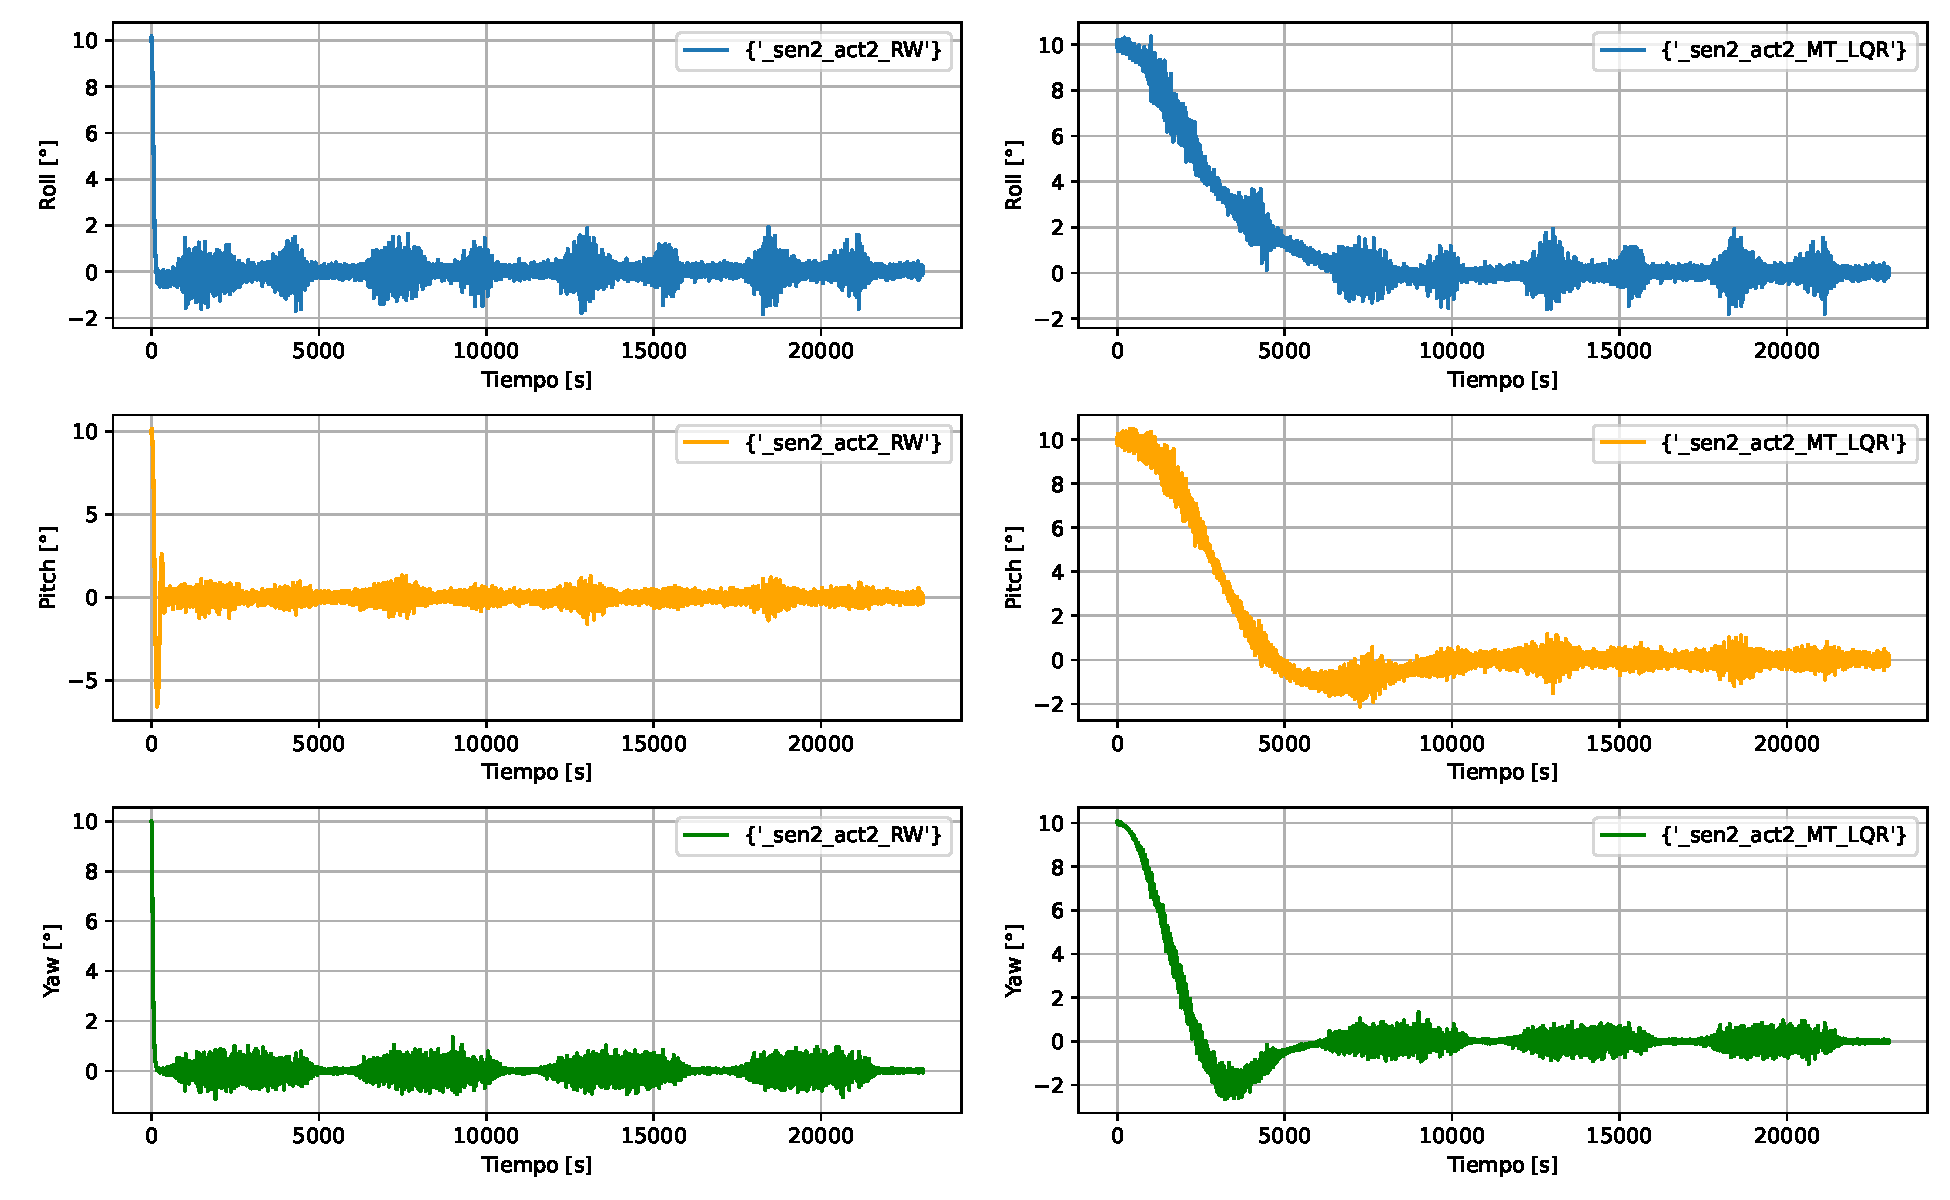
\includegraphics[width=0.97\textwidth]{MT_RW_nivel2.pdf}
	\caption{Ángulos de Euler LVLH y body para dos actuadores distintos (Elaboración propia).}
	\label{fig:MT_RW_nivel2}
\end{figure}

Además, en la Tabla~\ref{tab:RW_MT_nivel2} se observa de forma cuantitativa que las ruedas de reacción ofrecen mejores parámetros de rendimiento en términos de la norma de los MoP de apuntamiento, a cambio de un mayor consumo energético y una mayor masa en comparación con el uso de un solo actuador. Por lo tanto, según los requisitos de la misión, es fundamental que cada usuario evalúe qué opción resulta más adecuada en función de sus necesidades específicas.

\begin{table}[h!]
	\centering
	\caption{Rendimiento y costo para rueda de reaccion y magnetorquer en mismas condiciones.}
	\begin{tabular}{|c|c|c|c|c|c|}
		\hline
		\textbf{Tipo de}   & \textbf{Potencia} & \textbf{Masa [kg]} & \textbf{Accuracy [°]} & \textbf{Jitter} & \textbf{Agilidad [s]}  \\ 
		\textbf{actuador}   & \textbf{máxima [W]} & & & \textbf{[W/Hz]} &  \\
		\hline
		\textbf{Rueda de}   & 9  & 0.95  & 0.94 & 0.16 & 228   \\
		\textbf{reacción}   &  &   &  &  &    \\
		\hline
		\textbf{Magnetorquer}   & 0.8  & 0.053  & 1.71 & 0.42 & 3933   \\
		& & & & &   \\
		\hline
	\end{tabular}
	\label{tab:RW_MT_nivel2}
\end{table}


\subsubsection{Resultados de los controladores}

A continuación, se presenta un análisis comparativo entre el controlador PD y el controlador LQR aplicado al magnetorquer, con el objetivo de determinar cuál de estas opciones es más adecuada para su uso en la optimización.

En la Figura~\ref{fig:PD_LQR_nivel2}, se muestran los resultados de los ángulos de Euler llevados al equilibrio, utilizando sensores y actuadores de nivel medio (nivel 2). A la izquierda, se observa el control ejercido por el controlador PD, mientras que a la derecha, se presenta el control realizado por el controlador LQR. La Tabla~\ref{tab:PD_LQR_nivel2} resume los resultados de la norma de los MoP de apuntamiento.

La gráfica muestra que el controlador PD tarda más en estabilizar el sistema en el punto de equilibrio, utilizando los mismos componentes físicos (sensor de nivel medio y magnetorquer). Sin embargo, al estabilizarse más lentamente, se espera una mayor precisión en el apuntamiento, ya que el sistema permanece más tiempo alejado del punto de equilibrio dentro de la banda de asentamiento.

\begin{figure}[H]
	\centering    
	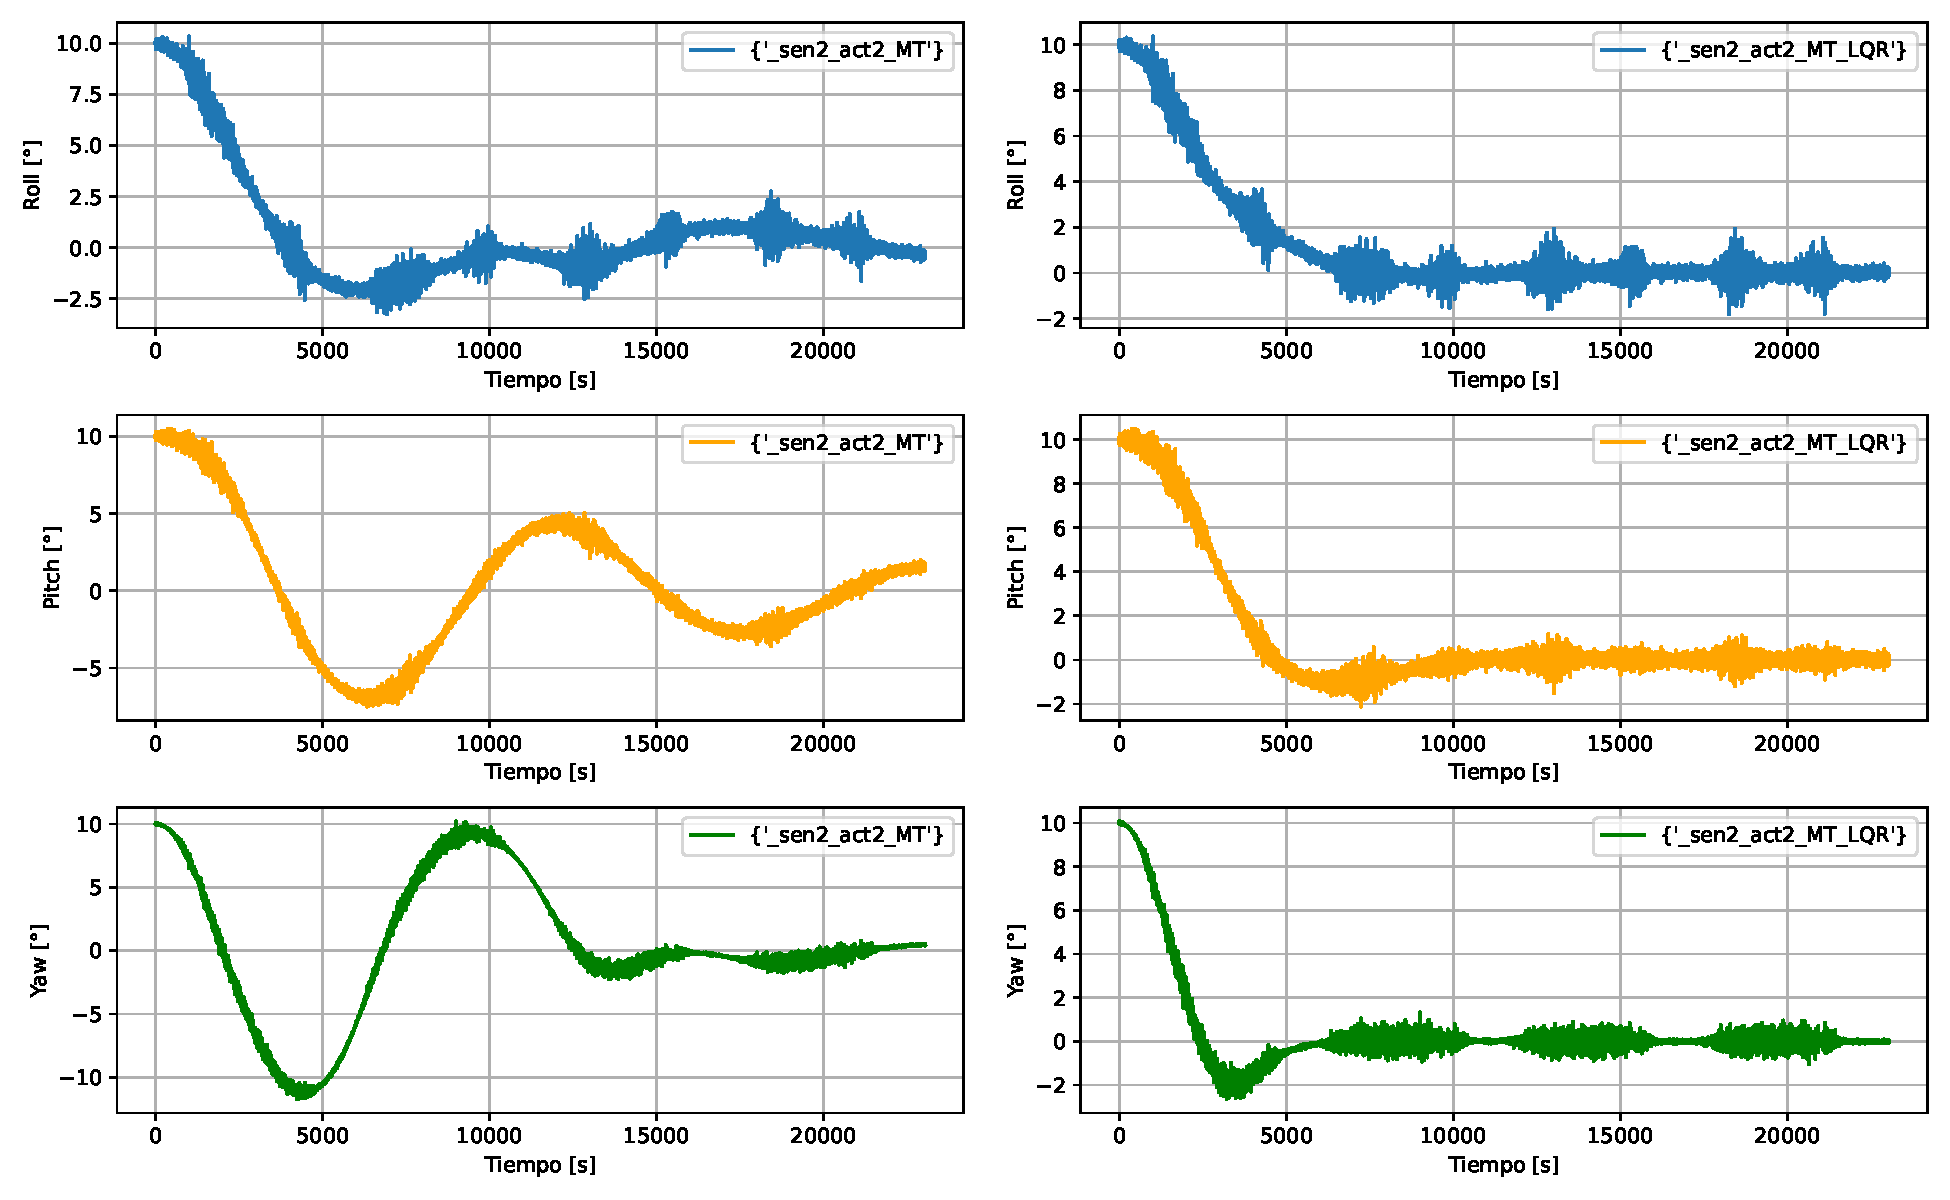
\includegraphics[width=0.97\textwidth]{PD_LQR_nivel2.pdf}
	\caption{Ángulos de Euler LVLH y body para dos controladores distintos (Elaboración propia).}
	\label{fig:PD_LQR_nivel2}
\end{figure}

Además, en la Tabla~\ref{tab:PD_LQR_nivel2} se confirma que, como se mencionó anteriormente, ambos controladores utilizan los mismos componentes, lo que implica el mismo consumo energético según la potencia máxima y la masa de los magnetorquers de nivel medio. Sin embargo, en términos de rendimiento, el controlador LQR ofrece un mejor tiempo de asentamiento y mayor precisión en el apuntamiento. Por esta razón, tanto para las ruedas de reacción como para los magnetorquers, se selecciona el controlador LQR para su implementación en la optimización dentro de la suite de simulación.

\begin{table}[h!]
	\centering
	\caption{Rendimiento y costo para controlador PD y LQR en mismas condiciones.}
	\begin{tabular}{|c|c|c|c|c|c|}
		\hline
		\textbf{Controlador}   & \textbf{Potencia} & \textbf{Masa [kg]} & \textbf{Accuracy [°]} & \textbf{Jitter} & \textbf{Agilidad [s]}  \\ 
		  & \textbf{máxima [W]} & & & \textbf{[W/Hz]} &  \\
		\hline
		\textbf{PD}   & 0.8  & 0.053  & 2.46 & 0.43 & 14040   \\
		&  &   &  &  &    \\
		\hline
		\textbf{LQR}   & 0.8  & 0.053  & 1.71 & 0.43 & 3933   \\
		& & & & &   \\
		\hline
	\end{tabular}
	\label{tab:PD_LQR_nivel2}
\end{table}

\subsubsection{Resultados niveles de sensores}

A continuación, se presenta un análisis sobre los tres niveles de sensores, utilizando actuadores de nivel 2 (medio), con el fin de evaluar cómo la estimación de la actitud del satélite, basada en los diferentes niveles de sensores, afecta los MoP de apuntamiento y su costo asociado.

En la Figura~\ref{fig:MT_LQR_sensores}, se muestran tres columnas de gráficas que representan el control de los ángulos de Euler hacia el equilibrio. En la primera columna, a la izquierda, se observa la simulación de actitud basada en los ángulos de Roll, Pitch y Yaw utilizando sensores de nivel 1 (bajo). La segunda columna muestra el caso con sensores de nivel 2 (medio), mientras que la tercera columna, a la derecha, corresponde a sensores de nivel 3 (alto). La Tabla~\ref{tab:MT_LQR_sensores} resume los resultados de los MoP de apuntamiento junto con los costos asociados a los distintos niveles de magnetómetro y sensor solar.

En la gráfica, se puede observar que, con sensores de nivel bajo, existe mayor ruido y dispersión en los ángulos de Euler una vez estabilizados en el equilibrio. Este comportamiento mejora conforme se incrementa el nivel de los sensores, mostrando una menor dispersión en los ángulos de Euler, lo que resulta en una mejora de la precisión de apuntamiento y una reducción del jitter.

\begin{figure}[H]
	\centering    
	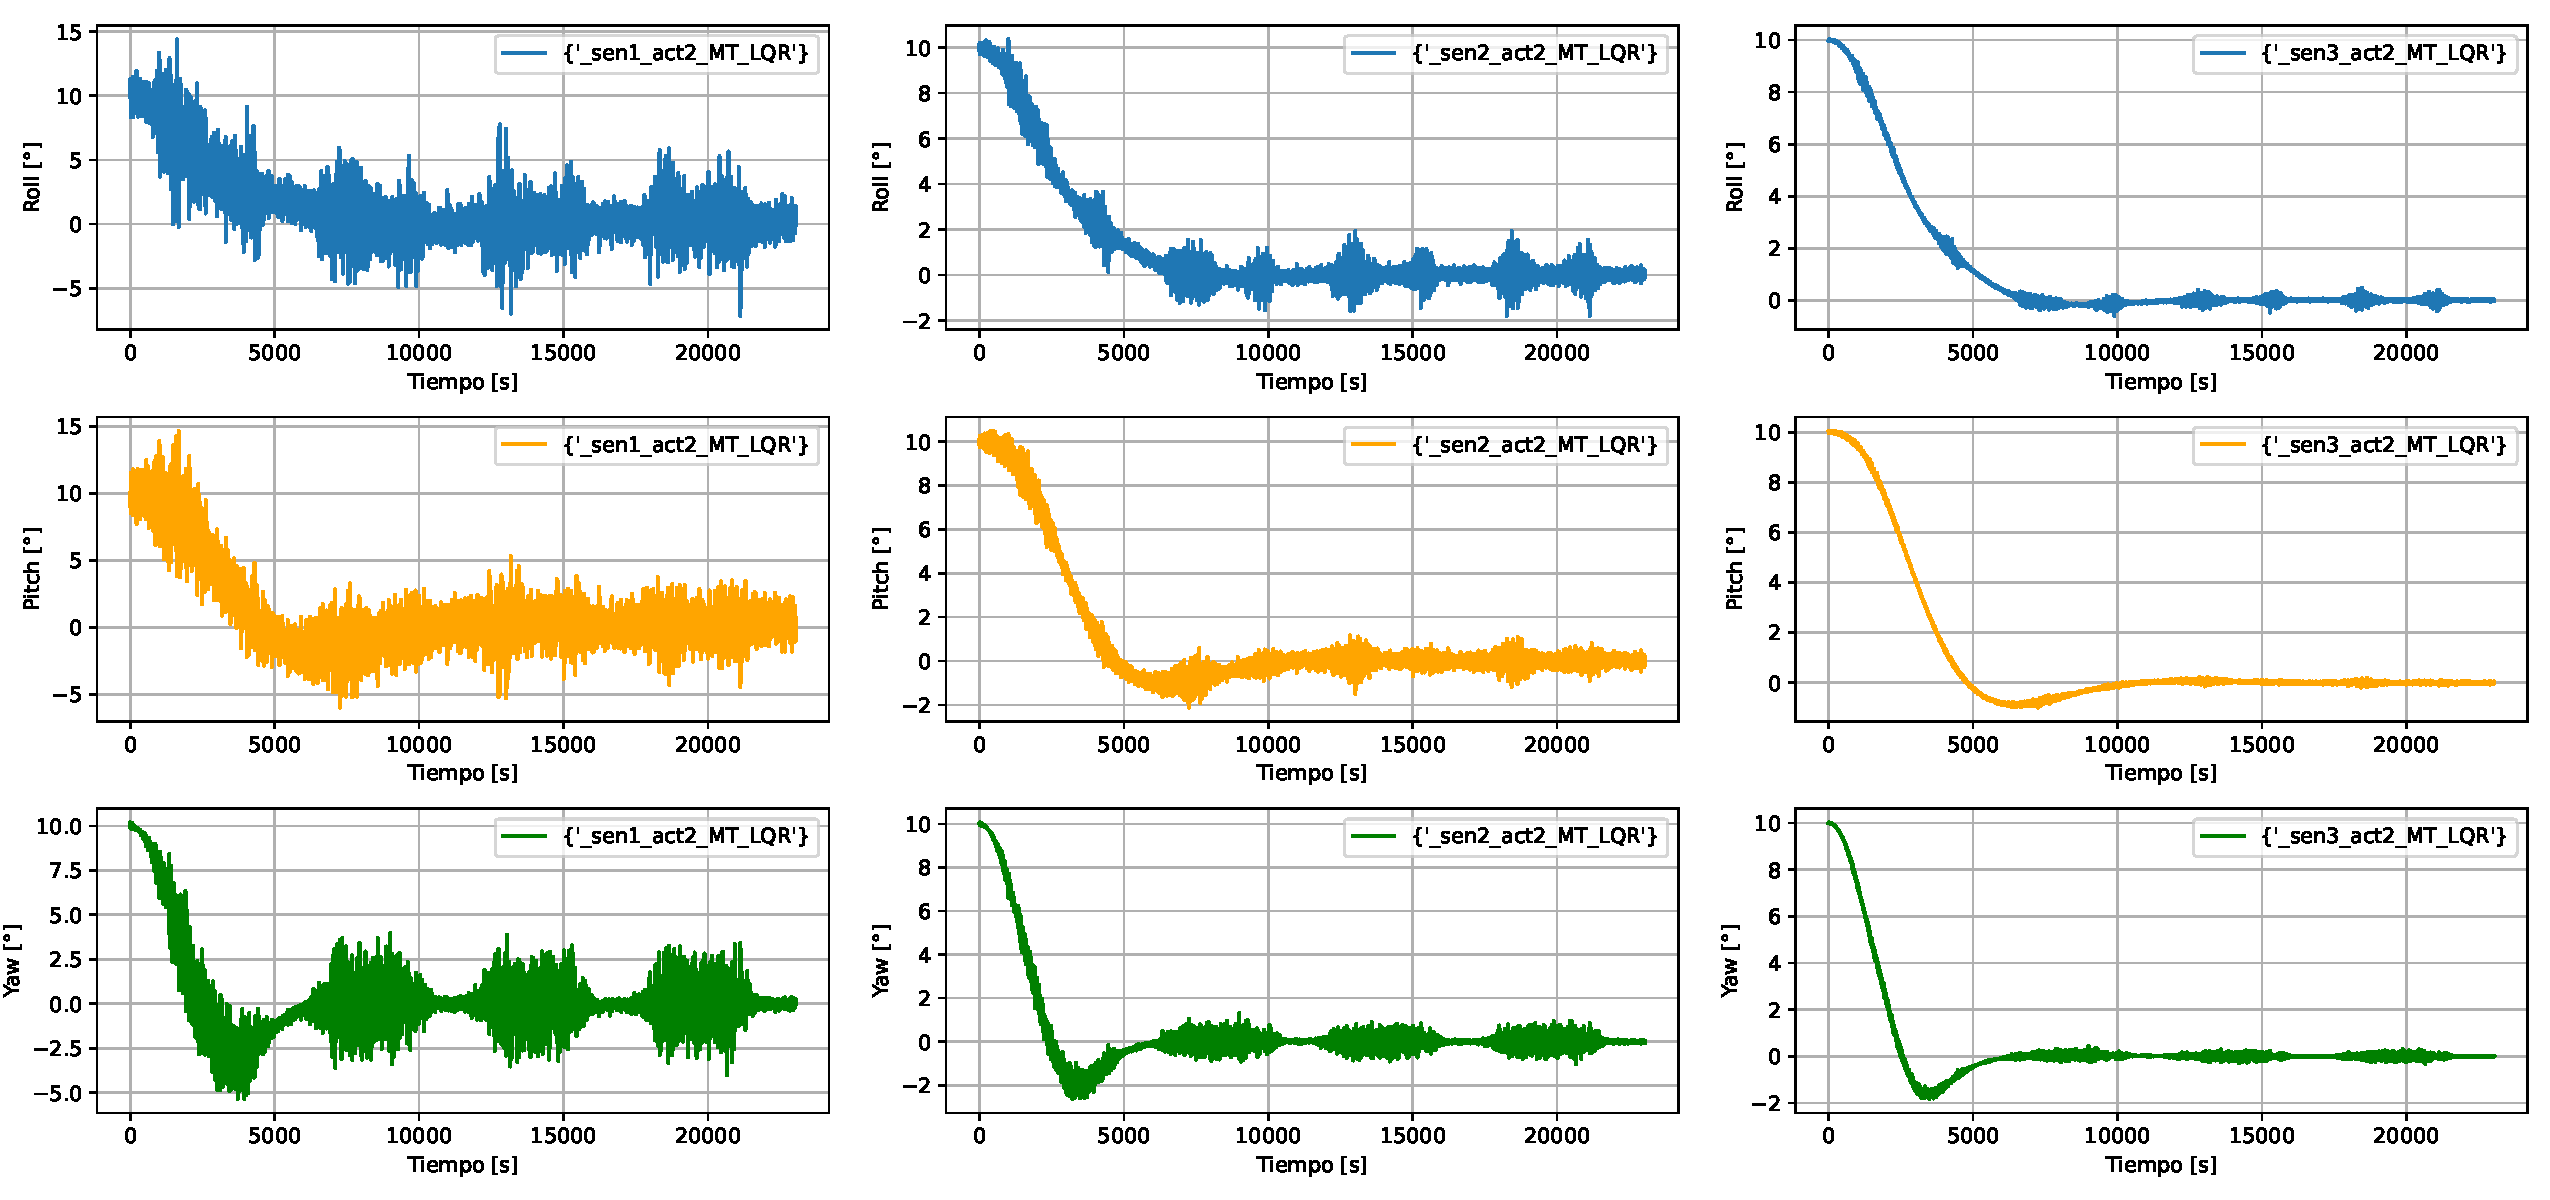
\includegraphics[width=0.97\textwidth]{MT_LQR_sensores.pdf}
	\caption{Ángulos de Euler LVLH y body para niveles de sensor distintos con magnetorquer (Elaboración propia).}
	\label{fig:MT_LQR_sensores}
\end{figure}

Además, en la Tabla~\ref{tab:MT_LQR_sensores} se confirma que la mejora en el nivel de los sensores contribuye significativamente a un mejor rendimiento en la precisión de apuntamiento y en la reducción del jitter. Sin embargo, una observación importante es que, aunque el paso de sensores de nivel medio a nivel alto mejoró la exactitud de apuntamiento, no tuvo un impacto notable en la reducción del jitter. En cuanto a la agilidad, el efecto de los sensores en la mejora del tiempo de asentamiento fue mínimo, lo que indica que este componente físico no está directamente relacionado con dicho MoP de apuntamiento.

\begin{table}[h!]
	\centering
	\caption{Rendimiento y costo para niveles de sensor con nivel 2 de magnetorquer y LQR.}
	\begin{tabular}{|c|c|c|c|c|c|}
		\hline
		\textbf{Nivel de}   & \textbf{Potencia} & \textbf{Masa [kg]} & \textbf{Accuracy [°]} & \textbf{Jitter} & \textbf{Agilidad [s]}  \\ 
		\textbf{sensor}  & \textbf{máxima [W]} & & & \textbf{[W/Hz]} &  \\
		\hline
		\textbf{Nivel 1}   & 0.15  & 0.067  & 3.72 & 2.92 & 4081   \\
		&  &   &  &  &    \\
		\hline
		\textbf{Nivel 2}   & 0.3  & 0.181  & 1.71 & 0.43 & 3933   \\
		& & & & &   \\
		\hline
		\textbf{Nivel 3}   & 0.75  & 0.530  & 1.5 & 0.43 & 3957   \\
		& & & & &   \\
		\hline		
	\end{tabular}
	\label{tab:MT_LQR_sensores}
\end{table}

En la Figura~\ref{fig:RW_LQR_sensores} se presenta el mismo análisis de sensores, pero en este caso utilizando las ruedas de reacción como actuador de nivel 2. También se muestran los resultados de los MoP de apuntamiento y el costo asociado a los sensores en la Tabla~\ref{tab:RW_LQR_sensores}.

En la gráfica, al igual que con los magnetorquers, se puede observar un mayor ruido y dispersión en los datos de los ángulos de Euler cuando se utilizan sensores de nivel bajo. Esta dispersión disminuye a medida que se incrementa la calidad de los magnetómetros y los sensores solares, evidenciándose una menor variabilidad en los datos una vez que se alcanza el equilibrio.

\begin{figure}[H]
	\centering    
	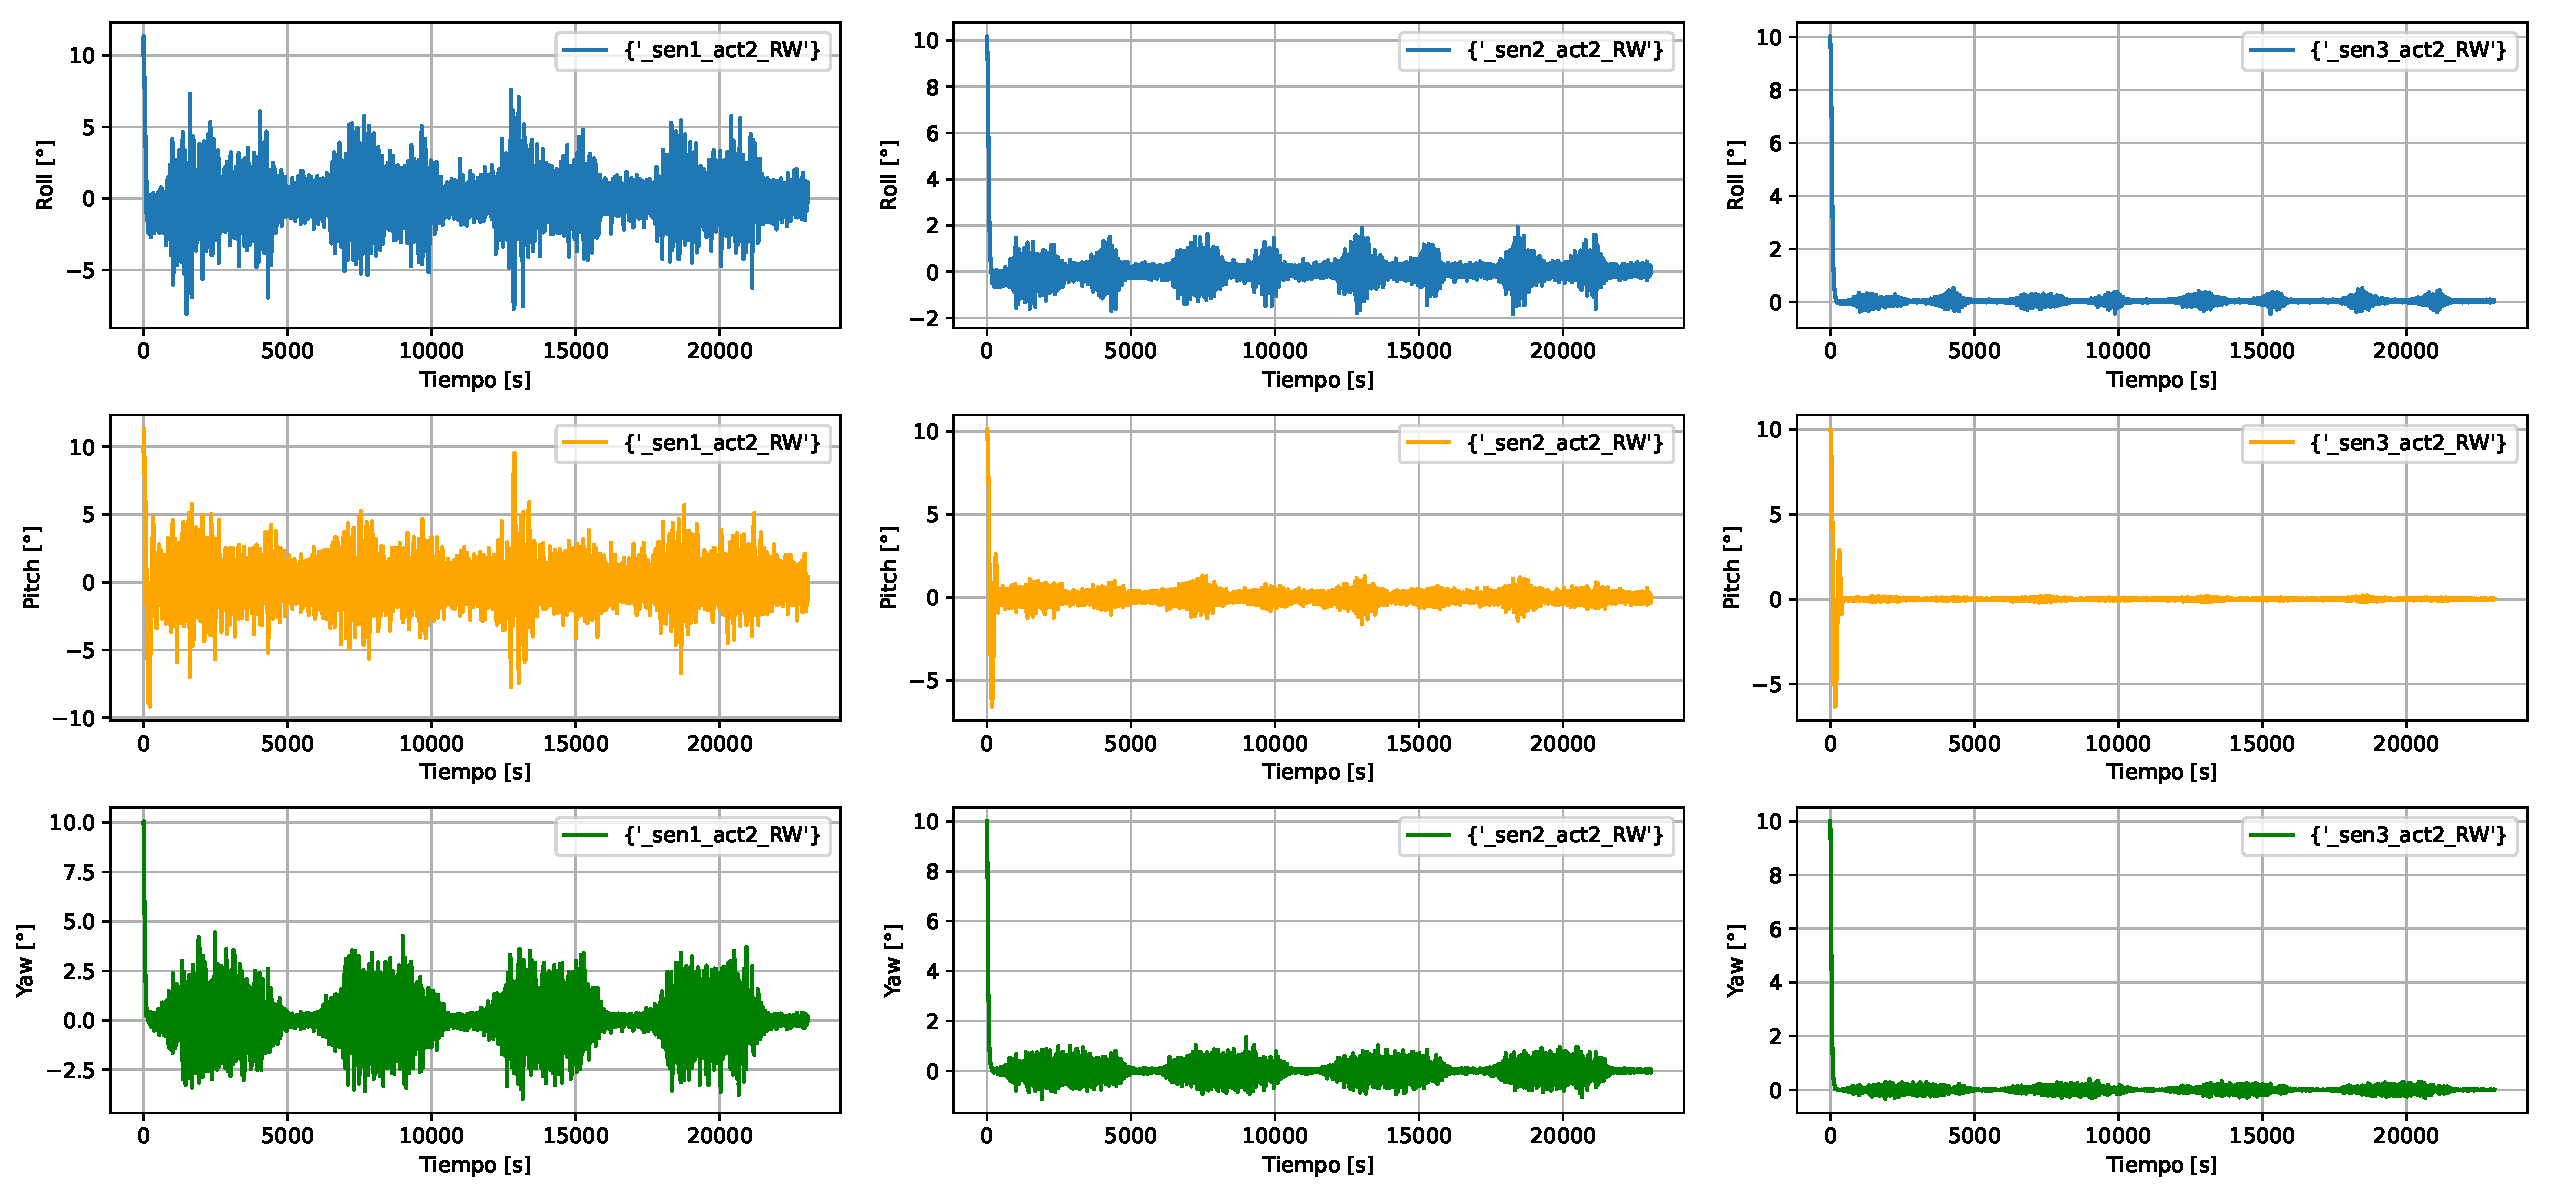
\includegraphics[width=0.97\textwidth]{RW_LQR_sensores.pdf}
	\caption{Ángulos de Euler LVLH y body para niveles de sensor distintos con rueda de reacción (Elaboración propia).}
	\label{fig:RW_LQR_sensores}
\end{figure}

En la Tabla~\ref{tab:RW_LQR_sensores}, se confirma lo mencionado anteriormente: se observa una mejora notable en la exactitud de apuntamiento y en el jitter al pasar de sensores de nivel bajo a medio, aunque esto conlleva un incremento significativo en el consumo de potencia y energía debido al uso de sensores de mayor calidad.

Un aspecto particular del caso de las ruedas de reacción es que, a diferencia de lo observado con los magnetorquers, en cada nivel se manifiesta una mejora en el jitter. En el caso de los magnetorquers, no se notó esta mejora al pasar del nivel 2 al nivel 3, donde los valores se mantuvieron constantes. Además, no se observa una mejora en la agilidad al incrementar el nivel de los sensores, como se evidencia en la tabla, donde los tiempos de asentamiento permanecen sin variaciones a pesar de la mejora en el componente físico.

\begin{table}[h!]
	\centering
	\caption{Rendimiento y costo para niveles de sensor con nivel 2 de rueda de reacción y LQR.}
	\begin{tabular}{|c|c|c|c|c|c|}
		\hline
		\textbf{Nivel de}   & \textbf{Potencia} & \textbf{Masa [kg]} & \textbf{Accuracy [°]} & \textbf{Jitter} & \textbf{Agilidad [s]}  \\ 
		\textbf{sensor}  & \textbf{máxima [W]} & & & \textbf{[W/Hz]} &  \\
		\hline
		\textbf{Nivel 1}   & 0.15  & 0.067  & 3.76 & 3.28 & 230  \\
		&  &   &  &  &    \\
		\hline
		\textbf{Nivel 2}   & 0.3  & 0.181  & 0.93 & 0.16 & 228   \\
		& & & & &   \\
		\hline
		\textbf{Nivel 3}   & 0.75  & 0.530  & 0.52 & 0.02 & 229   \\
		& & & & &   \\
		\hline		
	\end{tabular}
	\label{tab:RW_LQR_sensores}
\end{table}

\subsubsection{Resultados niveles de actuadores}

A continuación, se presentan análisis sobre los tres niveles de actuadores, utilizando sensores de nivel 2 (medio), para evaluar cómo la estimación de la actitud del satélite, en función de los diferentes niveles de actuadores, afecta los MoP de apuntamiento y su costo asociado.

En la Figura~\ref{fig:MT_LQR_actuadores}, se muestran tres columnas de gráficas que representan el control de los ángulos de Euler hacia el equilibrio. En la primera columna, a la izquierda, se presenta la simulación de actitud basada en los ángulos de Roll, Pitch y Yaw, utilizando magnetorquers de nivel 1. Las segunda y tercera columnas muestran el mismo análisis para los niveles 2 y 3, respectivamente. La Tabla~\ref{tab:MT_LQR_actuadores} resume los resultados de los MoP de apuntamiento y el costo asociado a los magnetorquers.

En la gráfica, se puede observar que, con actuadores de nivel bajo, el control es más suave, ya que el sistema tarda más tiempo en asentarse en el equilibrio. Sin embargo, esta situación mejora al utilizar magnetorquers de mayor calidad, como se evidencia en las otras dos columnas. Este comportamiento de mejora en el control hacia el equilibrio se aprecia con mayor claridad en la gráfica correspondiente al Yaw (verde).

\begin{figure}[H]
	\centering    
	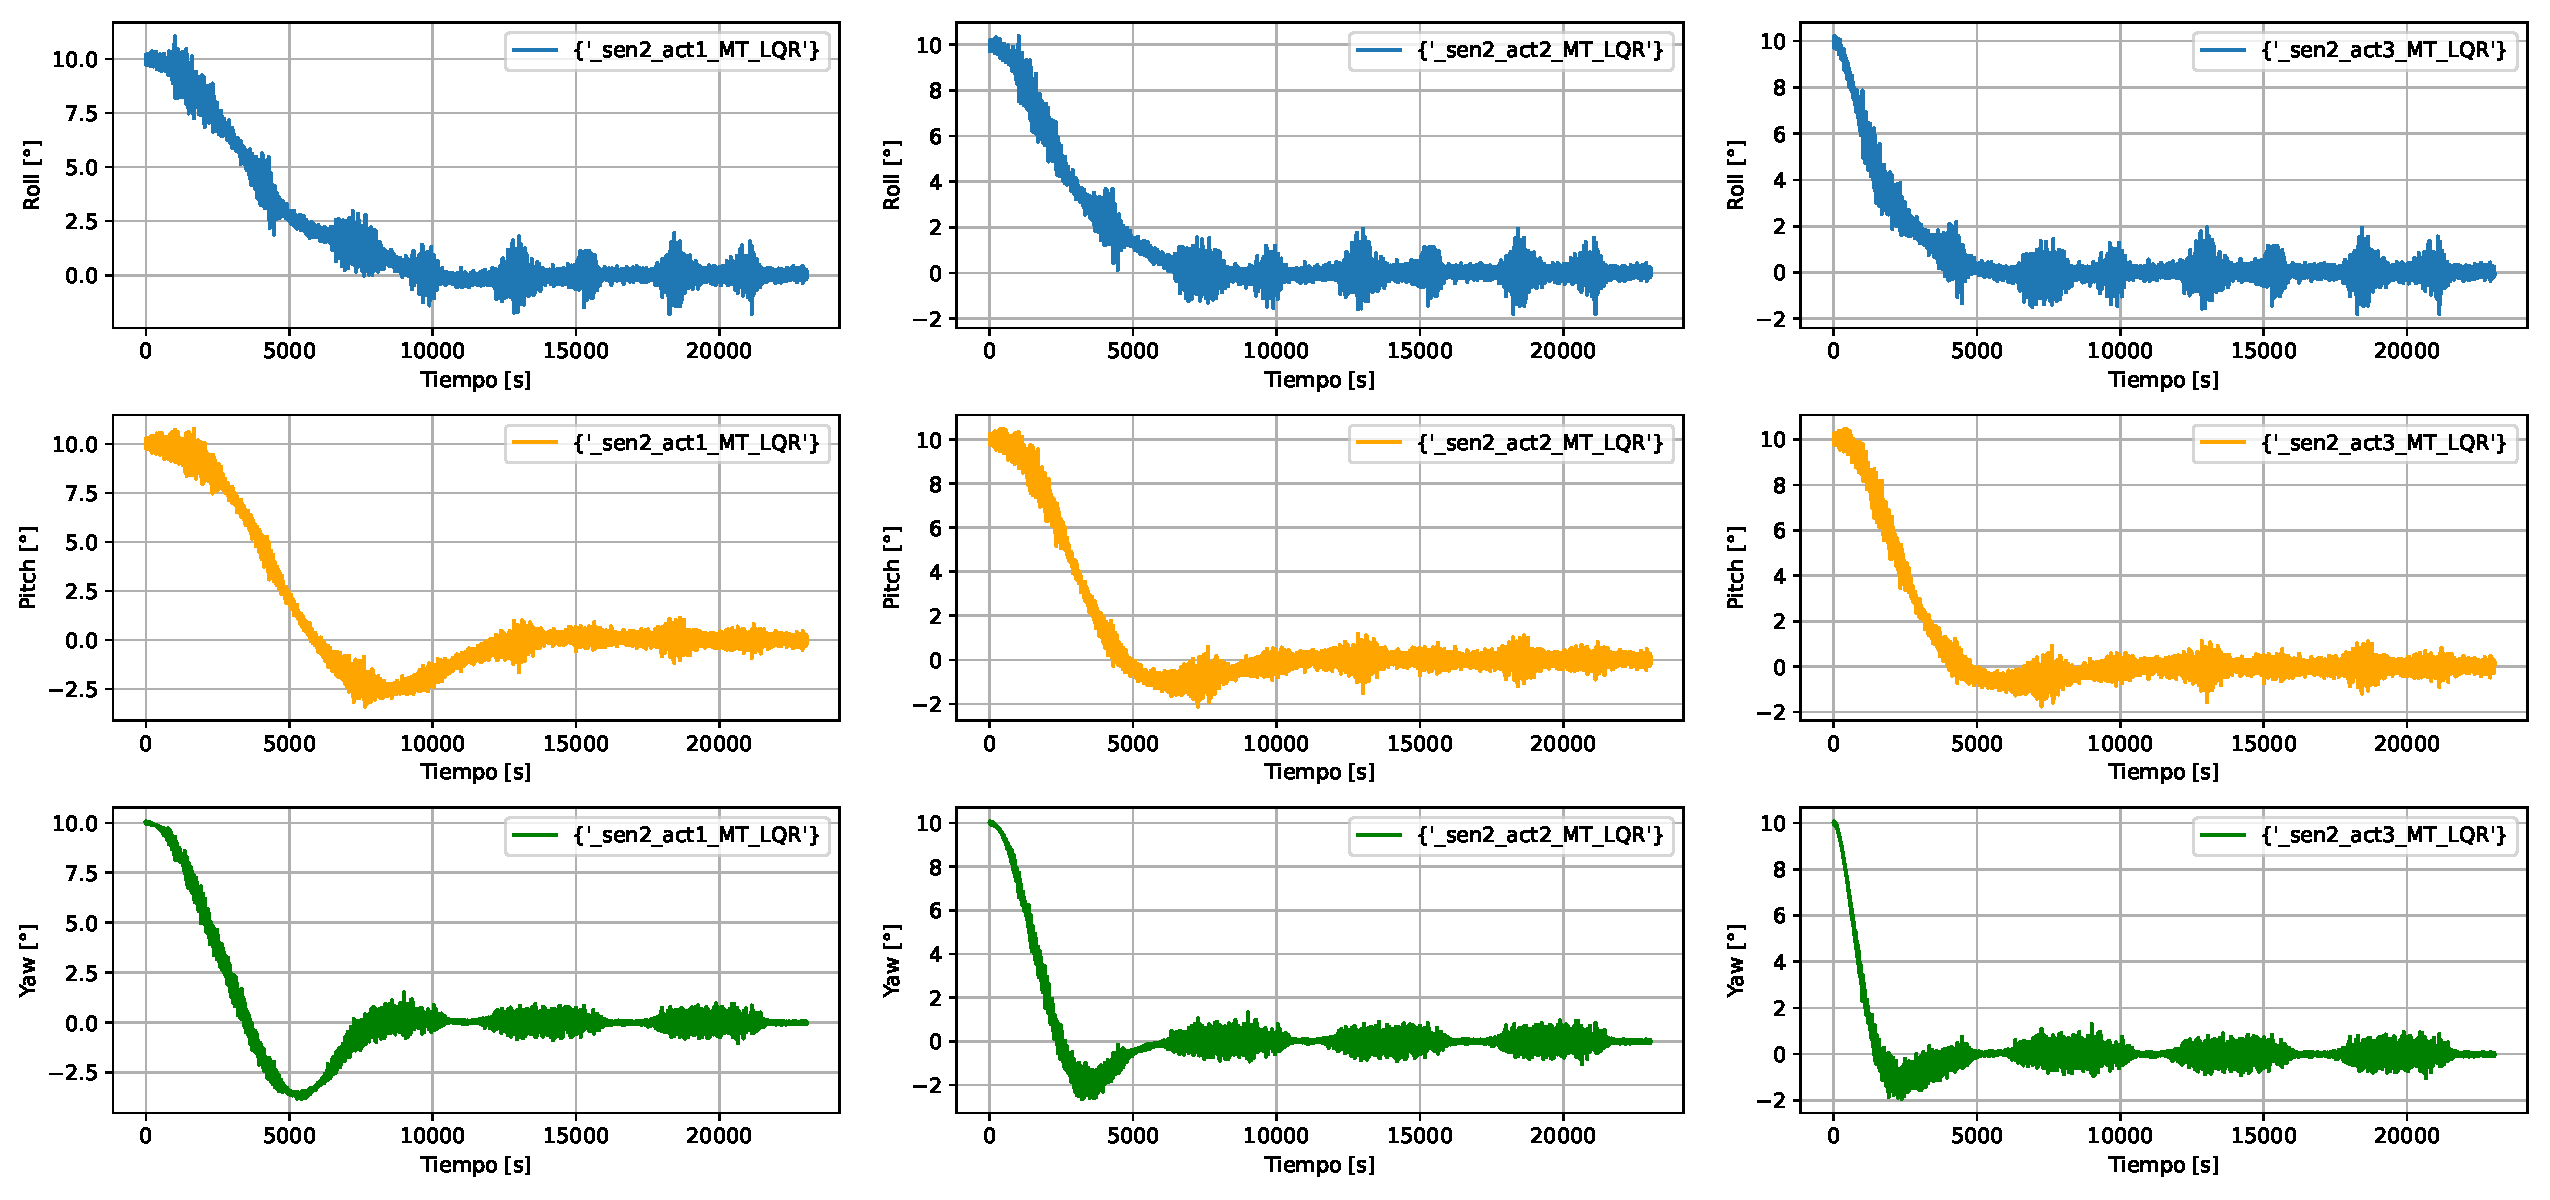
\includegraphics[width=0.97\textwidth]{MT_LQR_actuadores.pdf}
	\caption{Ángulos de Euler LVLH y body para niveles de magnetorquer distintos con sensores nivel 2 (Elaboración propia).}
	\label{fig:MT_LQR_actuadores}
\end{figure}

En la Tabla~\ref{tab:MT_LQR_actuadores}, se observa que, a medida que se incrementa el nivel de los magnetorquers, la norma de la exactitud de apuntamiento mejora del nivel 1 al nivel 2, pero se deteriora al alcanzar el nivel 3. También se nota una disminución en el tiempo de asentamiento, un aspecto que se representa de manera más clara en la gráfica.

Sin embargo, al aumentar el nivel del magnetorquer, se evidencia un incremento en el ruido, reflejado por el jitter. Este fenómeno se debe a que un mayor torque debido al campo magnético, genera vibraciones mecánicas que afectan la densidad espectral de potencia. A partir de los resultados, se puede concluir que existe una tendencia clara que indica que los magnetorquers están directamente relacionados con la mejora del tiempo de asentamiento. Sin embargo, es importante destacar que, dependiendo del caso, este aumento en el nivel del actuador puede no necesariamente traducirse en una mejora de la exactitud de apuntamiento, lo que sugiere que no hay una relación directa entre ambas variables en todas las situaciones.

\begin{table}[h!]
	\centering
	\caption{Rendimiento y costo para niveles de magnetorquer con nivel 2 de sensor y LQR.}
	\begin{tabular}{|c|c|c|c|c|c|}
		\hline
		\textbf{Nivel de}   & \textbf{Potencia} & \textbf{Masa [kg]} & \textbf{Accuracy [°]} & \textbf{Jitter} & \textbf{Agilidad [s]}  \\ 
		\textbf{actuador}  & \textbf{máxima [W]} & & & \textbf{[W/Hz]} &  \\
		\hline
		\textbf{Nivel 1}   & 0.275  &  0.03  & 3.09 &  0.41 & 5821   \\
		&  &   &  &  &    \\
		\hline
		\textbf{Nivel 2}   & 0.8  & 0.053  & 1.71 & 0.43 & 3933   \\
		& & & & &   \\
		\hline
		\textbf{Nivel 3}   & 1.11  & 0.43  & 1.83 & 0.49 & 2692   \\
		& & & & &   \\
		\hline		
	\end{tabular}
	\label{tab:MT_LQR_actuadores}
\end{table}

En la Figura~\ref{fig:RW_LQR_actuadores}, se presenta el mismo análisis aplicado a las ruedas de reacción, utilizando nuevamente sensores de nivel 2. Además, los resultados de los MoP de apuntamiento y el costo asociado a los actuadores se detallan en la Tabla~\ref{tab:RW_LQR_actuadores}.

En la gráfica, se observa un comportamiento similar al observado en el caso de los magnetorquers. A medida que se mejora el nivel del actuador, se evidencia una mejora en el control hacia el tiempo de asentamiento en los ángulos de Euler. Las gráficas muestran leves diferencias en la dispersión de datos y el ruido, lo que sugiere que, a simple vista, estos factores no afectan significativamente los demás MoP de apuntamiento analizados.

\begin{figure}[H]
	\centering    
	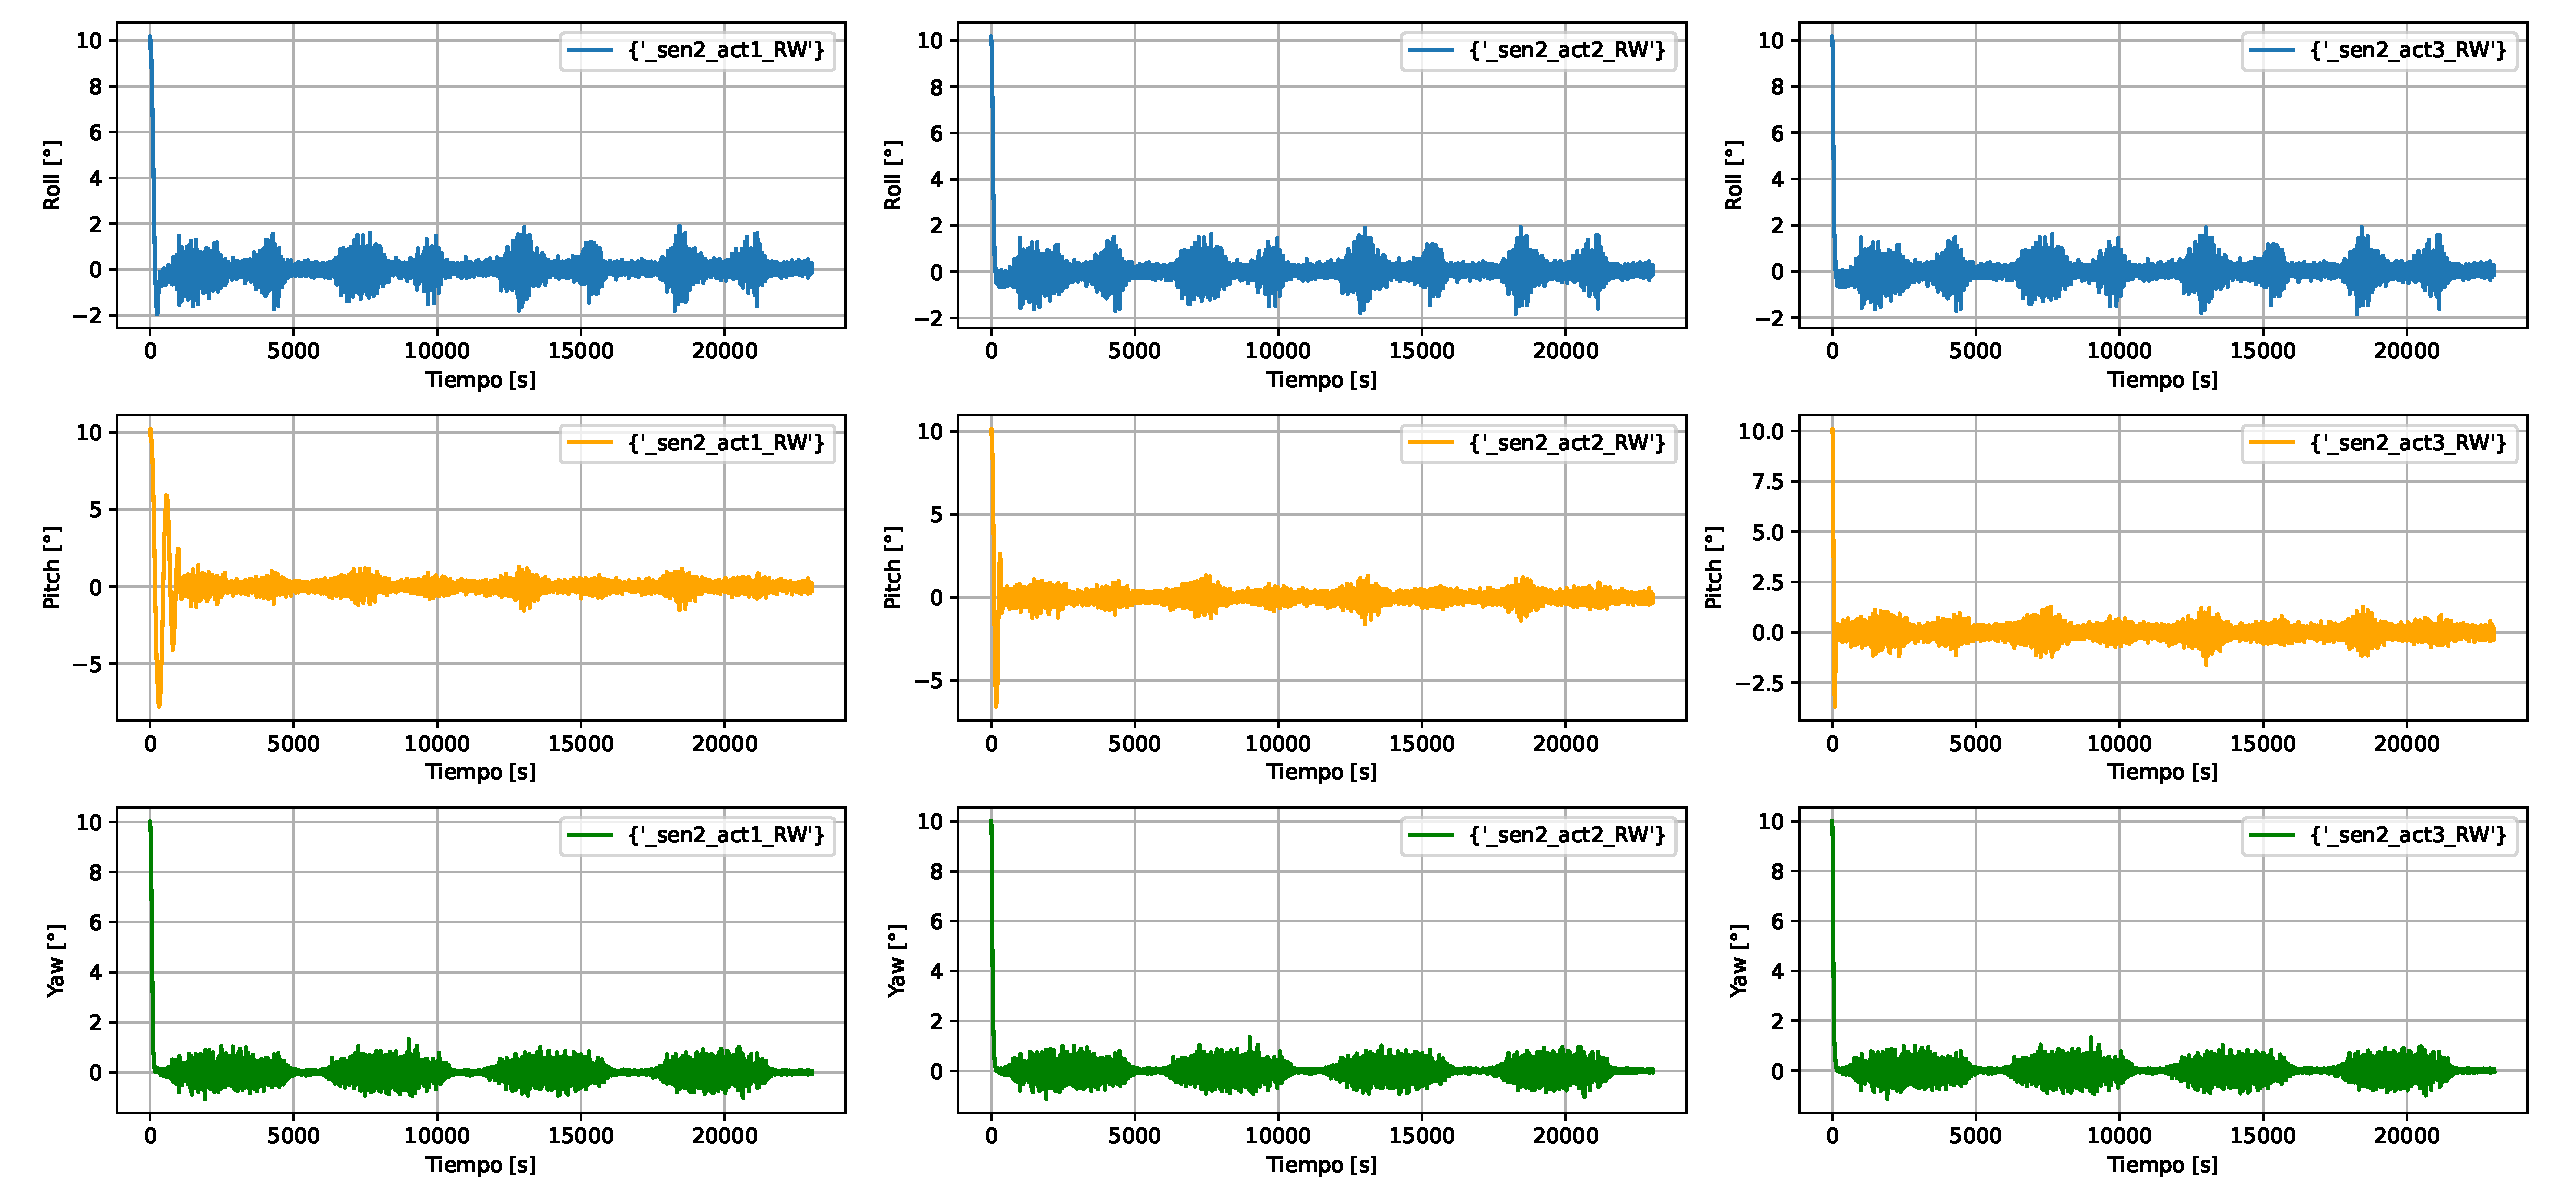
\includegraphics[width=0.97\textwidth]{RW_LQR_actuadores.pdf}
	\caption{Ángulos de Euler LVLH y body para niveles de rueda de reacción distintos con sensores nivel 2 (Elaboración propia).}
	\label{fig:RW_LQR_actuadores}
\end{figure}


En la Tabla~\ref{tab:RW_LQR_actuadores}, se puede observar que una mejora en el nivel de las ruedas de reacción implica un costo significativamente mayor, especialmente en comparación con los magnetorquers. Este aumento de costo se traduce en una mejora en el tiempo de asentamiento, así como en una mejora del jitter y, en menor medida, en la exactitud de apuntamiento. Sin embargo, es importante señalar que, a pesar de la mejora en el nivel de las ruedas de reacción, el impacto en la exactitud de apuntamiento no es significativo, lo cual se refleja también en las gráficas.

\begin{table}[h!]
	\centering
	\caption{Rendimiento y costo para niveles de rueda de reacción con nivel 2 de sensor y LQR.}
	\begin{tabular}{|c|c|c|c|c|c|}
		\hline
		\textbf{Nivel de}   & \textbf{Potencia} & \textbf{Masa [kg]} & \textbf{Accuracy [°]} & \textbf{Jitter} & \textbf{Agilidad [s]}  \\ 
		\textbf{sensor}  & \textbf{máxima [W]} & & & \textbf{[W/Hz]} &  \\
		\hline
		\textbf{Nivel 1}   & 6  & 0.75  & 1.18 & 0.36 & 628  \\
		&  &   &  &  &    \\
		\hline
		\textbf{Nivel 2}   & 9  & 0.95  & 0.93 & 0.16 & 228   \\
		& & & & &   \\
		\hline
		\textbf{Nivel 3}   & 10  & 3.2  & 0.95 & 0.15 & 63   \\
		& & & & &   \\
		\hline		
	\end{tabular}
	\label{tab:RW_LQR_actuadores}
\end{table}

\subsection{Resumen sobre análisis realizados}

Al analizar los resultados obtenidos con la suite de simulación, se pueden establecer las siguientes conclusiones:

\begin{itemize}
	\item \textbf{Rueda de reacción vs Magnetorquer:} A partir de los análisis realizados y el examen detallado de ambos actuadores, se concluye que las ruedas de reacción ofrecen un mejor rendimiento, especialmente en términos de exactitud de apuntamiento y reducción del tiempo de asentamiento. Por otro lado, se recomienda el uso de magnetorquers para misiones con menos restricciones en el rendimiento o con mayores limitaciones en alguno de los SE envelopes, ya que su costo es inferior.
	
	\item \textbf{PD vs LQR:} Este análisis se llevó a cabo para determinar la viabilidad de utilizar un controlador PD en las optimizaciones, en comparación con el LQR para ambos actuadores. Los resultados mostraron que el LQR siempre superó al PD en términos de exactitud de apuntamiento y tiempo de asentamiento, por lo que se optó por la segunda opción.
	
	\item \textbf{Análisis del nivel de sensores:} Se buscó entender cómo el tipo de sensores impacta en los parámetros de rendimiento para asignar un peso específico a las variables de optimización. Se observó que los sensores mejoran significativamente la exactitud de apuntamiento y reducen el jitter, aunque no hay una relación clara con la agilidad, que mostró poca variación. Esta tendencia es consistente tanto para las ruedas de reacción como para los magnetorquers.
	
	\item \textbf{Análisis del nivel de actuadores:} Similar al análisis de sensores, se buscó establecer una relación entre el nivel de los actuadores y los parámetros de rendimiento. Se encontró que ambos actuadores ofrecían mejores valores de agilidad, con un tiempo de asentamiento reducido a medida que mejoraba el actuador. Sin embargo, el jitter aumentaba con el mejoramiento del magnetorquer debido a las interacciones mecánicas y magnéticas dentro del CubeSat, a diferencia de las ruedas de reacción. No se observó una relación clara entre la exactitud de apuntamiento y los niveles medio y alto, aunque se confirmó que los actuadores de nivel bajo resultan en una menor exactitud de apuntamiento.
\end{itemize}


